\chapter{SENSOR NETWORKS BACKGROUND} 
\label{cha:Sensor Networks/Data Aggregation/Security Background}
	
	Sensor networks are becoming ubiquitous in our day to day life. 
	It is a scenario in which network and computers are extremely inexpensive objects and they are surrounded to real people all the time \cite{2002-Stajano-ubiquitous}.	
	In this chapter, we introduce sensor networks and its applications, we define basic terminologies and then we discuss major 
	barriers to achieve security in sensor networks.

\section{Applications}
	In sensor networks, thousands of sensor nodes may interact with the physical world and collectively monitor an area, generating a large amount of data to be transmitted and reasoned about.
	With the recent advances in hardware technologies of sensors, we can use tiny and cheap sensor nodes to obtain significant amount of useful data about physical world.
	For example, we can use them to discover temperature, water quality, lightning condition, humidity and pressure levels. 
	We can also use them to know certain characteristics of objects such as speed, direction, and size.
	% noise level, carbon dioxide level, oxygen level, soil moisture, magnetic field, 
	% the presence or absence of certain kinds of objects, and all kinds of values about machinery like mechanical stress level or movement \cite{hof2007applications}.
	These versatile types of sensors, allow us to use sensor network in a wide variety of scenarios.
	For example, sensor networks are used in military, environmental monitoring, health care, scientific data collection, emergency fire alarm systems, traffic monitoring, wildfire tracking, wildlife monitoring and many other applications.
	
	\begin{description}
		\item[Military Application]
			Sensor networks can be used for enemy tracking, battlefield surveillance or target classification \cite{li2002detection}.
			For example, \textit{Palo Alto Research Center} tries to spot ``interesting'' vehicles (the vehicles marked specially) using motes equipped with microphones or steerable cameras \cite{chu2004distributed}.
			The goal is to synchronize the sensor network to sense the track of a moving object with minimum information loss about the track of a moving object.

		\item[Environmental Monitoring] 
			Sensor networks can be utilized to monitor a geographical location. 
			For example, \textit{Meteorology and Hydrology in Yosemite National Park} \cite{lundquist2003meteorology}, a sensor network was deployed to monitor the water system across and within the Sierra Nevada.
			The goal was to collect the data and derive information on natural climate fluctuation caused due to global warming.
			It also provided information on the increasing needs of water consumers.
			Research of the water system in the Sierra Nevada is difficult, because of its geographical structure.
			Sensor networks can be very useful in such situations as they can operate with little or no human intervention.
		
		\item[Health Care]
			Sensors can be used to monitor the patients around the clock. 
			They can report various statistics to the doctors and nurses regarding patients health.
			Also, it can send reminders to them to take care of the patient periodically. 	
			The most important criteria for the such networks are security and reliability.
			Because based on the sensor readings, doctors decide what treatment or what medicine to prescribe to the patients.
			If those readings are modified by an adversary then the consequences might be lethal to the patients.

		\item[Sustainable Mobility]
			Sensor networks can be used to build digitally connected and coordinated vehicles.
			With the driver less cars from companies like Google, autonomous vehicle systems seems the future of transportation.
			Autonomous vehicle systems \cite{benenson2008towards} describes how various various technologies in addition to the sensor networks is used in making the sustainable mobility.
		
		\item[The Active Floor]
			is a system which can detect person walking on the floor using pressure sensors \cite{addlesee1997orl}.
			It also allows to extract information from the raw sensor data which has reasonable success in identifying people based on their gait.
			Authors used Hidden Markov Models based analysis techniques originally developed for speech and face recognition to identify people.
		
		% \item[Code Blue]
		% 	is a system to enhance emergency medical care with the goal to have a seamless patient transfer between a disaster area and a hospital\cite{lorincz2004sensor}.
	\end{description}
	
	The applications of the sensor networks are enormous. 
	The application platform of a sensor network determines the design of the sensor nodes, the network protocol and security architecture.
	As far as we know, there is no general architecture for such design.
	Therefore, developing a protocol for sensor networks can certainly be challenging. 

\section{Sensor Node Architecture}
	Sensor networks consists of an individual sensor node and the construction of each node depends on the application.
	The major components of the sensor nodes are shown in Figure \ref{fig:sensor-node-architecture} \cite{karl2007protocols}.
	\begin{figure}[h!]
		\centering
		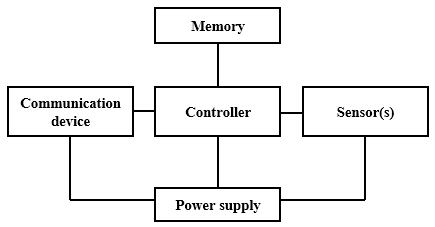
\includegraphics{images/sensor-node-architecture.png}
		\caption{Sensor Node Block Diagram}
		\label{fig:sensor-node-architecture}
	\end{figure}

	\begin{description}
	\item[Controller] is the Central Processing Unit (CPU) of the node.
		It is responsible for collecting data from the sensors and processing it to deriving useful information from it. 
		It also decides nodes for end to end communications and affects the actuator's behavior.
		It executes variety of  algorithms, ranging from time-critical signal processing and communication protocols to application algorithms.
	
	\item[Communication Device] is utilized for trans receiving data between end hosts at radio frequency.
		Radio Frequency(RF)-based communication is widely used in sensor networks.
		RF based communications does not require line of sight between sender and receiver.
		It also provides relatively long range communications capabilities and high data rates.
		It has an acceptable error rates at reasonable energy consumption.
		All these characteristics, best fits the requirements of many sensor network applications.
		The most important function for the communication devices is to convert a bit stream to radio waves. 
		% It is convenient to use a device that combines these two tasks in a single entity, called transceivers. 
		% Usually, half-duplex operation is realized since transmitting and receiving at the same time on a wireless medium is impractical in most cases.

	\item[Sensors] are the nodes generating raw data to be transmitted and analyzed by the network.
		% It can be temperature, pressure, light, humidity or gas sensor depending on the application.
		% The sensors can be either \textit{Passive} or  \textit{Active}.
		\textit{Passive sensors} can measure a physical quantity without affecting the environment at the point of deployment. 
		For example, vibration, chemical sensors sensitive for given substances and smoke detectors.
		\textit{Active sensors} actively probes the environment and generates raw information to be analyzed.
		For example, a radar sensor or some types of seismic sensors creates shock waves by small explosions into the sea to get the details about the earth.  
		These are very specific explosions and requires quite special permissions to carry out such experiments.

	\item[Power Supply of Sensor Nodes] is an important system component, too.
		Sensor nodes can be powered by using normal AA battery which stores about 2.2 - 2.5 Ah at 1.5 V.
		To increase the longevity of the nodes and wireless sensor networks we can use energy from a node’s environment ``energy scavenging''.
		% For example, \textit{Vibrations} is almost pervasive form of mechanical energy: walls or windows in buildings are resonating with cars or trucks passing in the streets, machinery often has low frequency vibrations, ventilations also cause it, and so on.
		% The available energy depends on both amplitude and frequency of the vibration.
		% \textit{Pressure variations} is similar to vibrations, a variation of pressure can also be used as a power source. 
		% Such piezoelectric generators are in fact used already. 
		% One well-known example is the inclusion of a piezoelectric generator in the heel of a shoe, to generate power as a human walks about \cite{shenck2001energy}. 
		% This device can produce, on average, 330 $\mu W / cm^{2}$. 
		For example, \textit{Photovoltaics} effect is used in the solar cells, can be applied to power supply module of the sensor nodes.
		\textit{Temperature gradients} effect utilizing the differences in temperature can be converted to electrical energy and can be used to power sensor nodes.

	\item[The Memory Component] is fairly straightforward. 
		Random Access Memory (RAM) can be used to store sensor readings, and temporary data. 
		The operating system code can be stored in Read-Only Memory (ROM). 
		It is important to dimension RAM and ROM precisely, to reduce the manufacturing cost and power consumption.
	\end{description}

\section{Energy Consumption}

	The sensor network's lifetime can be maximized by minimizing the power consumption of communication devices or trans-receiver of the sensor nodes.
	The trans receiver is responsible for all the wireless communications between nodes.
	To estimate the power consumption, we have to consider the communication and computation power consumption.
	The trans receiver's energy dissipation depends on two main parameters \cite{wang2002energy}.
	The first is $E_{elec} (J/b)$, the energy dissipated to run the transmit or receive electronics.
	The second is $\varepsilon_{amp} (J/m^2 b)$, the energy dissipated by the transmit power amplifier to achieve an acceptable signal to noise ratio $E_{b} / N_{o} $ at the receiver.
	We assume the $d^2$ energy loss for transmission between sensor nodes since the distances between sensors are relatively short \cite{ettus1998system}. 
	To transmit a $k$ - bit packet at distance $d$, the energy dissipated is:
	\begin{equation}
		E_{tx}(k, d) = E_{elec} \cdot k + \varepsilon_{amp} \cdot k \cdot d^{2}
	\end{equation}
	and to receive the k - bit packet, the radio expends
	\begin{equation}
		E_{rx}(k) = E_{elec} \cdot k
	\end{equation}
	For $\mu Amp$\ wireless sensor, $E_{elec} = 50nJ/b$\ and $\varepsilon_{amp} = 100pJ/m^2 b$.

	Trans receiver can be put into different states to save energy \cite{karl2007protocols}.
	It can be in either transmit or receive state and energy consumption of those states are describe above.
	It can be in Idle state where it is ready to receive packet but is not currently receiving anything.
	It can be in Sleep state where majority of the parts are switched off, and is not able to receive immediately. 
 	To sustain the sensor network for longer times all aspects of the sensor network should be efficient.
	For example, the networking algorithm for routing should be such that it minimizes the distance $d$\ between the nodes.
	The signal processing algorithm should be such that it process the networking packets with less computations.
	It is shown in \cite{wang2002energy} that by using Fast Fourier Transform (FFT) algorithm in the devices requires less communication between the sensor nodes.
	To minimize the energy dissipation, a processor should operate at the lowest possible voltage for a given clock frequency.

\section{Resource Constraints}
	\label{sec:aggregate-adversary}
	We introduce the parameters which should be taken into account while designing secure protocol for sensor networks.  
	These parameters can constrain the protocol designer's choices within the protocol.

	\subsection{Physical Limitations}
		Sensor nodes are often used in open, hostile and unattended environments.
		They are vulnerable to physical attacks due to the lack of physical security available in their environment.
		It allows an adversary to gain the secret information from a compromised sensor node.
		An adversary can reprogram the sensor node with virus(malicious software).
		The compromised node then report an arbitrary false sensor readings to its parent node in the tree hierarchy, making the sensor readings unreliable and irrelevant	.
		These attacks become more damaging when multiple adversaries succeeds in injecting false data into the network which may cause catastrophic consequences \cite{wagner2007algorithms}.	

	\subsection{Hardware Limitations}
		As far as we know, one of the first hardware platform for developing sensor network application is MICA \cite{hill2002mica} developed by University of Berkeley.
		Another popular platform is Mote from Intel \cite{arazi2006self}.
		Due to lower manufacturing cost of sensor nodes, they have low speed processor, limited storage, a short range trans receiver.
		For example, the major specifications for the latest ZigBee chip supporting IEEE 802.15.4 standard, CC2538 from Texas Instruments are shown in Table \ref{table:soc}.
		This chip can do most of the security algorithms but has really little amount of memory storage. It has limited output power which constraints its transmission range which forces us to use multi-hop routing in the network as one node can not communicate with the node outside of its transmission range.
		These hardware limitations can constrain protocol designer's choice of algorithms for applications.  
		\begin{table}[!htb]	
			\begin{center}
			 	\caption{System-on-Chip specifications for CC2538 from Texas Instruments implementing IEEE 802.15.4 standards}
				\label{table:soc}
				\begin{tabular}{ |l| l| }
					% \hline
				     % & CC2538 \\
				    \hline
				    Device Type & Wireless Micro controller \\
				    Frequency & 2.4GHz \\
				    Processor Integration & ARM Cortex-M3 \\
						Flash & Up to 512 KB \\
						RAM & Up to 32 KB \\
						Security & AES-128/256; SHA2; RSA \\
						RX Current & 20 (mA) \\
						Output Power & 7 (dBm) \\
						Data Rate(Max) & 250 kbps \\
						Type of Battery & AAA; AA; Rechargable(Li-ION) \\
				    \hline
				\end{tabular}
			\end{center}
		\end{table}
	
	\subsection{Transmission Medium}
		In sensor networks, a group of sensor nodes (or processors) communicate over the radio (e.g., Blue-tooth, WLAN).
		Traditionally, wireless mediums have issues due to synchronization, hidden station and expose station terminal problems, distributed arbitration, directional antennas, bandwidth limitations, higher error rate, security, scalability etcetera.
		For example, wireless networks have approximately $10^6$ times higher bit error rate (BER) than wired networks which causes frequent link loss and then path loss. 
		Hence, making unstable routing in the network.
		Higher BER creates higher collision rate in the network, generating higher overhead of retransmission and lowering the channel utilization and the throughput of the network.
		This kind of transmission medium with constrained resources makes it challenging to design the reliable networking protocol as we have to consider all the possible retransmissions.

	\subsection{Mobility}
		As we know, sensor nodes communicate via radio and the availability of the transmission medium changes over time due to link failure, bandwidth limitations or change in network topology.
		Nodes may be mobile creating the instability of the network link, which require the reconfiguration and special protocol to redesign the network.
		The mobility issue makes difficult to do the routing in the network with the directional antennas in place.
		It also requires network to be agile enough to do the reconfiguration for the newer network topology.
		It impedes while doing the quality of service in the network. 
		
	All these parameters combined contributes to making strong assumptions on the network topology while designing the protocol for sensor networks.